\chapter{مقدمه}
\label{chap:intro}

\begin{figure}
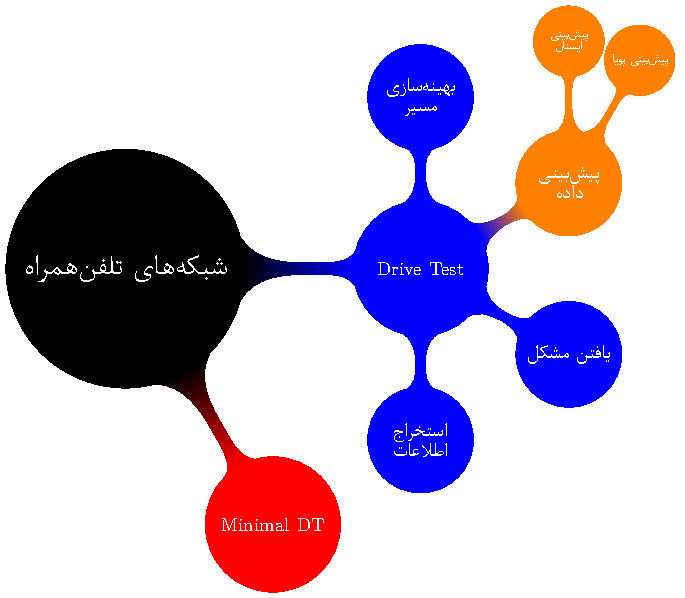
\includegraphics[width=\linewidth]{/ETCMobile/0GTo6G/mainFig}
\caption{\lofimage{/ETCMobile/0GTo6G/mainFig}
نسل‌های مختلف شبکه‌های تلفن‌همراه
}
\label{fig:0GTo6G}
\end{figure}
امروزه شاهد گسترش روزافزون شبکه‌های تلفن‌همراه در سرتاسر جهان هستیم. اطلاعات آماری حکایت از آن دارد که تا انتهای سال ۲۰۲۳ از میان 
$8.02$
میلیارد انسانی که بر روی کره زمین زندگی می‌کنند، در حدود 
$5.6$
میلیارد نفر از شبکه‌های تلفن‌همراه استفاده می‌کنند که این خود حاکی از
\gls{PenetrationCoefficient} $69$
درصدی این شبکه‌ها است. برطبق گزارش مؤسسه
\gls{GSMA}،
فناوری تلفن‌همراه و خدمات مرتبط با آن در سال 2023، در حدود 
$5.7$
تریلیون دلار ($5.4\%$ تولید ناخالص داخلی) ارزش‌افزوده به همراه داشته
\cite{GSMA2024MobileEconomy}.
این حجم شگرف چرخش مالی، منجر به ایجاد فرصت‌های پژوهشی، صنعتی و تجاری بسیاری گشته است. اهمیت شبکه‌های تلفن‌همراه، زمانی آشکار می‌گردد که بدانیم رشد و توسعه این شبکه‌ها، مرهون توسعه فناوری‌‌هایی نظیر 
\gls{MIMO}، \gls{IOT}، \gls{SDN}، \gls{NFV}و \gls{CloudComputing}
بوده است. این مهم به‌ویژه در شبکه‌های نسل پنج، بیش‌ازپیش خودنمایی می‌کند. 

شروع توسعه شبکه‌های نسل دو به‌مانند 
\gls{GSM}
در دهه 1980، با تمرکز بر ارائه خدماتی نظیر تبادل
\gls{Call} صوتی و \gls{SMS}
شکل گرفت. اما به‌مرور نقطه تمرکز به ارائه خدمات مبتنی بر 
\gls{PacketSwitch}
نیز معطوف گشت
(\gls{GPRS} و \lr{Edge}).
توسعه شبکه‌های نسل سه
\gls{UMTS}،
بسان پلی بود که ما را بیش‌ازپیش، بدین هدف نزدیک‌تر می‌نمود. در سال 2004، ایده‌های اولیه شبکه‌های نسل چهار 
(\gls{LTE} و \lr{LTE-Adv})،
با هدف ایجاد یک شبکه دسترسی با سرعت و ظرفیت بالا، قابلیت ارائه خدمات مختلف و انعطاف در تعامل با دیگر شبکه‌ها، تدوین گشت. در حال حاضر 
\lr{4G}
با سرعت سرسام‌آوری در حال توسعه جایگاه خویش در میان شبکه‌های تلفن همراه است، تا جایی که در سال 2018 در حدود 47 درصد کل ارتباطات تلفن همراه را به خود تخصیص داده است
\cite{globenewswire2019}. 




\gls{ITU} 
در پروژه‎ 
\lr{IMT-2020}، 
سه ویژگی کلیدی 
\lr{5G} 
را ارتباطات پرشمار ماشینی (مانند 
\lr{IoT})، 
پایدار و با 
\gls{Delay} 
اندک بر می‌شمارد. انتظار بر آن است که 
\lr{5G} 
از لحاظ پوشش، سرعت و تأخیر عملکرد چشمگیرتری نسبت به 
\lr{4G} 
از خود نشان دهد. برطبق نمودار 
\lr{Gartner} 
سرمایه‌گذاری و کار بر روی 
\lr{5G} 
حداقل تا یک دهه آینده ادامه خواهد داشت. تحقیقات بر روی شبکه‌های نسل جدید 
\lr{6G} 
از هم اکنون آغاز گشته و رد پای آن را در برخی از مقالات پژوهشی موجود در این حوزه می‌توان یافت 
(\autoref{fig:0GTo6G}).



\section{طرح مسئله}

\begin{ntdefinition}[\lr{QoS}]
	توانایی شبکه برای فراهم‌آوردن یک خدمت مشخص با یک سطح اطمینان معین را
 \gls*{QualityofService} (\gls*{QoS})
	می‌نامیم.
\end{ntdefinition}

\section{چالش‌ها و انگیزه}

\section{نوآوری‌ها}
نوآوری‌های این پایان‌نامه به طور خلاصه به شرح زیر است:
 \begin{itemize} 
 \tick 
ارایه یک روش نوین برای بهینه‌سازی ....
 \end{itemize}
 

\section{ساختار گزارش}
نخست در
\autoref{chap:concepts}،
تعاریف و مفاهیم مبنایی در حوزه‌ی شبکه‌های تلفن همراه مانند معماری 
\gls{UE}
بیان می‌شود. در
\autoref{chap:relatedworks}،
به معرفی و بررسی کارهای پیشین انجام شده در این حوزه پرداخته خواهد شد. در 
\autoref{chap:approach}،
روش پیشنهادی این پژوهش ارائه خواهد شد که شامل استفاده از داده‌های جمع‌آوری‌شده از \gls{DriveTest}، مدل‌سازی کانال، و به‌کارگیری روش‌های هوش مصنوعی برای پیش‌بینی دقیق‌تر و بهبود عملکرد شبکه است. در 
\autoref{chap:simulation}
نتایج به‌دست‌آمده از آزمایش‌های متعدد روش پیشنهادی را تحلیل کرده و در نهایت در
\autoref{chap:conclusion}
به جمع‌بندی این پژوهش خواهیم پرداخت.
